\chapter{Methodology}

\section{Participants}

A total number of \todo{26} participants, \todo{\# females and rest} with the average age of \todo{average age} with the standard deviation of \todo{sd age} took part in the experiment. The participants were all students of the University of Osnabrück. Before the start of the first exploration session all participant gave their written consent for taking part in the experiment (see appx. \ref{appx:forms}, Einverständniserklärung). The participation was voluntary and only students with no health issue were selected (see appx. \ref{appx:forms}, Anamnese). The participants were compensated by test-subject hours and/or 5€ per hour.  

Due to the Covid-19 pandemic sessions were conducted according to the laboratory hygiene regulations with a mask and under 3G rule.

3 participants were excluded due to not being able to comply with the experimental requirements, i.e., come in less than 3 days and more than 4 hours apart.



\section{Experimental Design}

\subsection{City}

This study is conducted in a virtual reality (VR) city with an area of about 1 km\textsuperscript2. The city is consisted of 284 buildings. 56 buildings are used in the experimental task of this study from which 4 are global landmarks, 26 are {\emphasize context meaningful} locations, e.g., shops, construction sites, and 26 are residential, {\emphasize not context meaningful} buildings. These 56 buildings have human agents in front of them and an artwork on one of their walls. Avatars belonging to shops take the pose of an act according to the functionality of that store {\emphasize(meaningful)}, e.g., has a book in the hand in front of a bookstore, or are just standing in front of the building {\emphasize(standing avatar)}. The artworks on the shops are also depicting the kind of the shop.

\todo{
	- FIG: include a map \\
	- include photos of the city
}

\subsection{Application and Technology}

The application of the experiment is implemented utilizing unity version 2019.4.11f1. The assets of the city, e.g., buildings, streets were obtained from a previous study called SpaRe, made also at the university of Osnabrück. They were modified with blender version 2.83 LTS (Long Term Support), as were also the human agents picked from Adobe Mixamo collection. They were modified for this experiment in a way that some contextual objects were added to the human agents in front of context meaningful buildings with regard to the context of the building. \\
The experiment consisted of two separate parts, i.e., Exploration and Testing.  Each part had the option to choose the language of the instructions, i.e., German and English. The experiment was conducted using a HTC Vive Pro Eye VR-Headset. For the virtual moving purposes inside the virtual city the participants were given Index valve controller to navigate inside a city by moving the joystick of the controller. They had both the right and left controllers to be able to use their dominant hand.

\section{Experimental Procedure}

For both parts of the experiments participants were seated on a backless rotating chair to enables them to physically rotate in the virtual city. Any forward, backward and sideways movement were done utilizing the controllers.

\subsection{Exploration}

The exploration consisted of 5 sessions. The sessions had to be no more than 3 days and no less than 4 hours apart. \\
The total duration of each session was 30 minutes broke down into 10 minutes segments for breaks to reduce the possibility of motion sickness. Before starting each segment the built-in eye-tracker of the VR-Headset was calibrated and validated. \\

After inserting participant-ID and choosing the preferred language of the participant the exploration session started with a tutorial. The tutorial was held in a scene separate from the main city. The purpose of the tutorial was to allow the participant to move around, get acquainted with the controller and practice the possible movement options the experiment allowed for. After participants confirmed their confidence in using the controllers the experiment was continued to the exploration session. In the main city participants were advised to explore the city freely.

\subsection{Testing}

No longer than 3 days and no less than 4 hours after the last exploration session the testing session was conducted. The testing comprised of just one session of approximately 2 hours. The testing starts after inputting the participant-ID and choosing the language. There is then a tutorial scene outside of the main city used in the experiment for participants to get acquainted with how to use the controller for performing the tasks. Before presenting the trials and in intervals of 112 trials eye-tracker was calibrated and validated. \\

The testing comprised 336 trials. There were 28 starting locations to perform the pointing task from in the city. The distribution of the starting locations can be seen in figure \ref{fig:starting_locs}. At each starting location 12 target buildings were randomly chosen from a pull of 112 targets (56 task buildings with and without avatars). Some examples are shown in figure \ref{fig:target_photos}. Each of the four conditions of the experiment, i.e., context meaningful with human agent present, context meaningful with no human agent present, non-context meaningful with human agent present, non-context meaningful with no human agent present built up 25\% of the trials.  The starting locations themselves were consistent for all participants and their order was randomized for each participant. All movements except the rotation were blocked for the whole testing session to maintain the consistence of the participants' position for in starting locations between participants. \\


\begin{figure}[h]
	\centering
	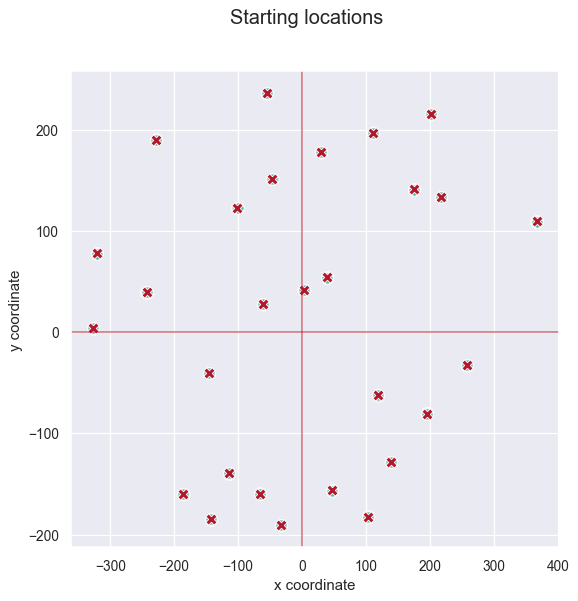
\includegraphics[width=80mm]{figures/starting_locations.png}
	\caption{distribution of the starting locations in the city.}
	\label{fig:starting_locs}
\end{figure}



\begin{figure}[h!]
	\centering
	\begin{subfigure}[b]{0.32\linewidth}
		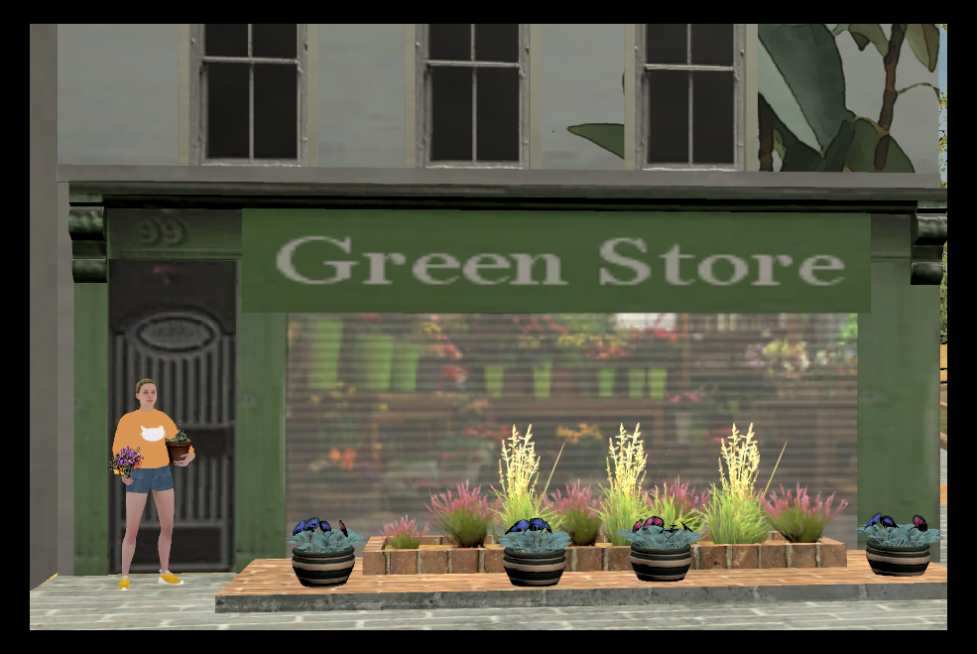
\includegraphics[width=\linewidth]{figures/45_S(green store)_A.PNG}
		\caption{shop with human agent}
	\end{subfigure}
	\begin{subfigure}[b]{0.32\linewidth}
		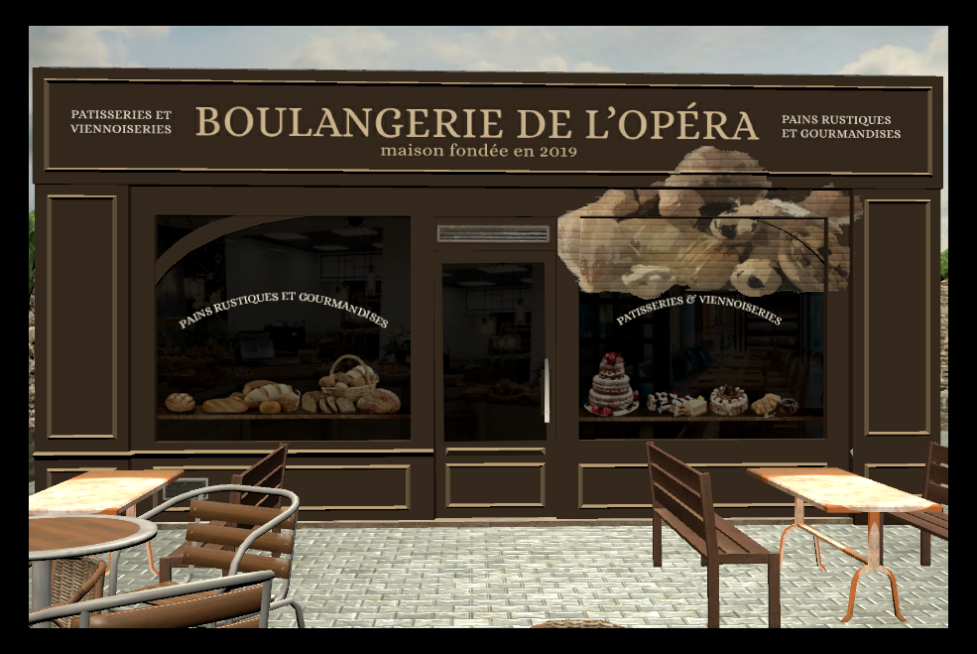
\includegraphics[width=\linewidth]{figures/02_S(boulangerie)_noA.PNG}
		\caption{shop without human agent}
	\end{subfigure}
	\begin{subfigure}[b]{0.32\linewidth}
		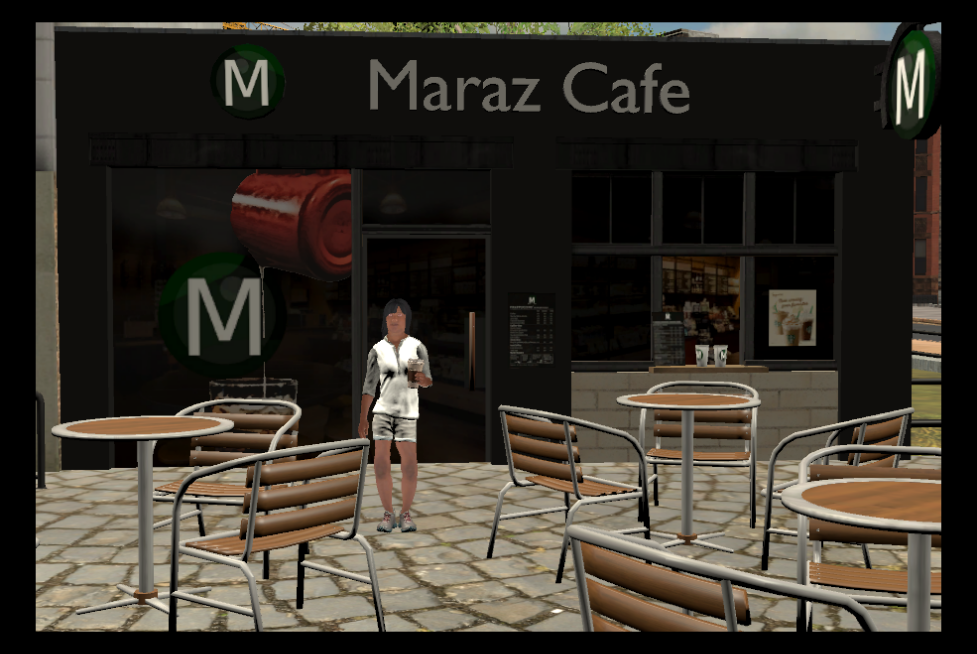
\includegraphics[width=\linewidth]{figures/05_S(Maraz cafe)_A.PNG}
		\caption{shop with human agent}
	\end{subfigure}
	
	\begin{subfigure}[b]{0.32\linewidth}
		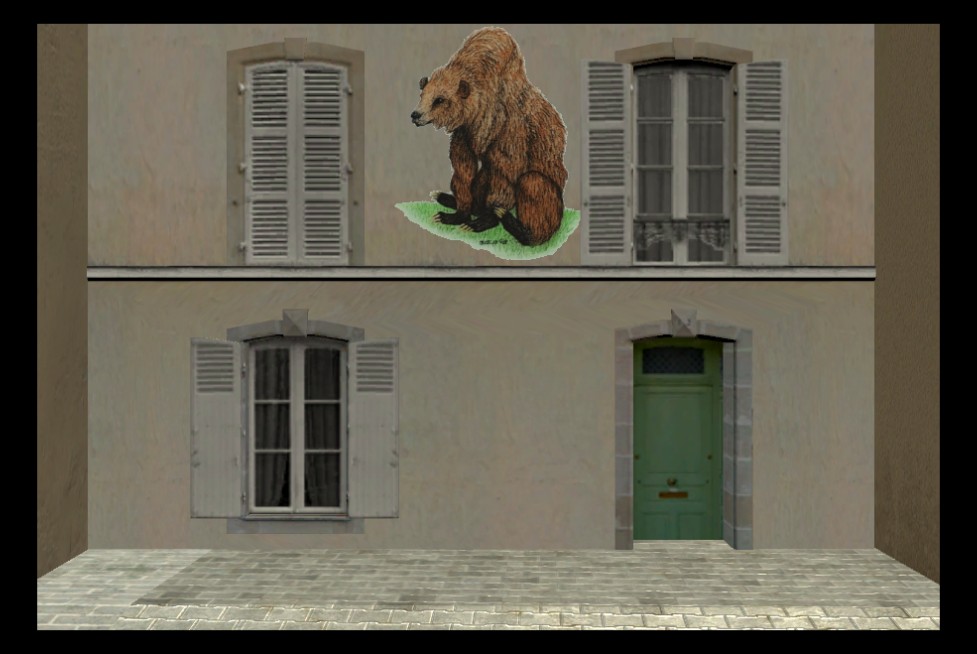
\includegraphics[width=\linewidth]{figures/07_R(bear)_noA.PNG}
		\caption{residential without human agent}
	\end{subfigure}
	\begin{subfigure}[b]{0.32\linewidth}
		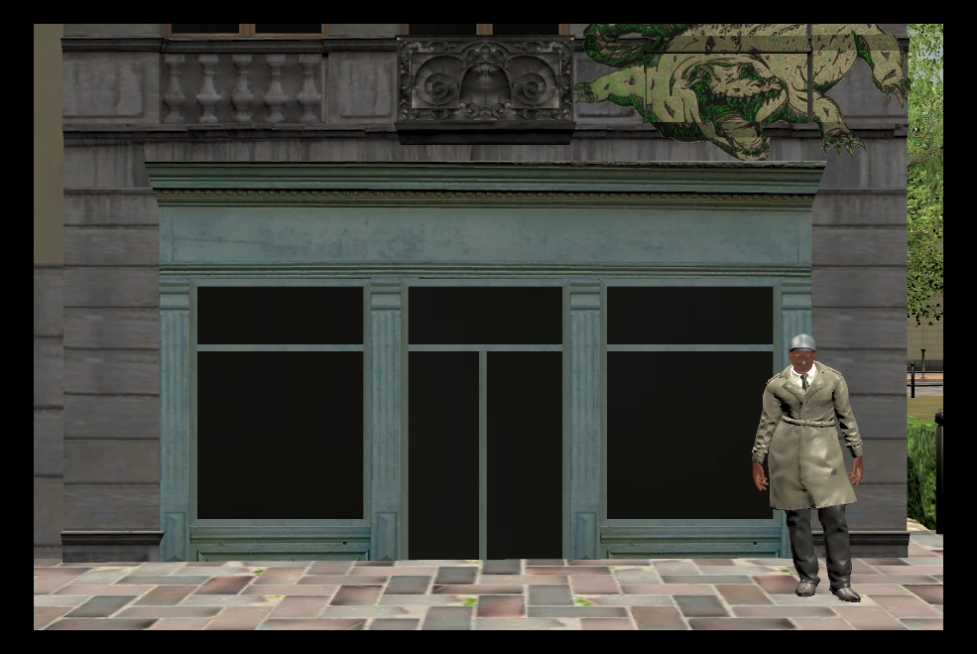
\includegraphics[width=\linewidth]{figures/25_R(alogator)_A.PNG}
		\caption{residential with human agent}
	\end{subfigure}
	\begin{subfigure}[b]{0.32\linewidth}
		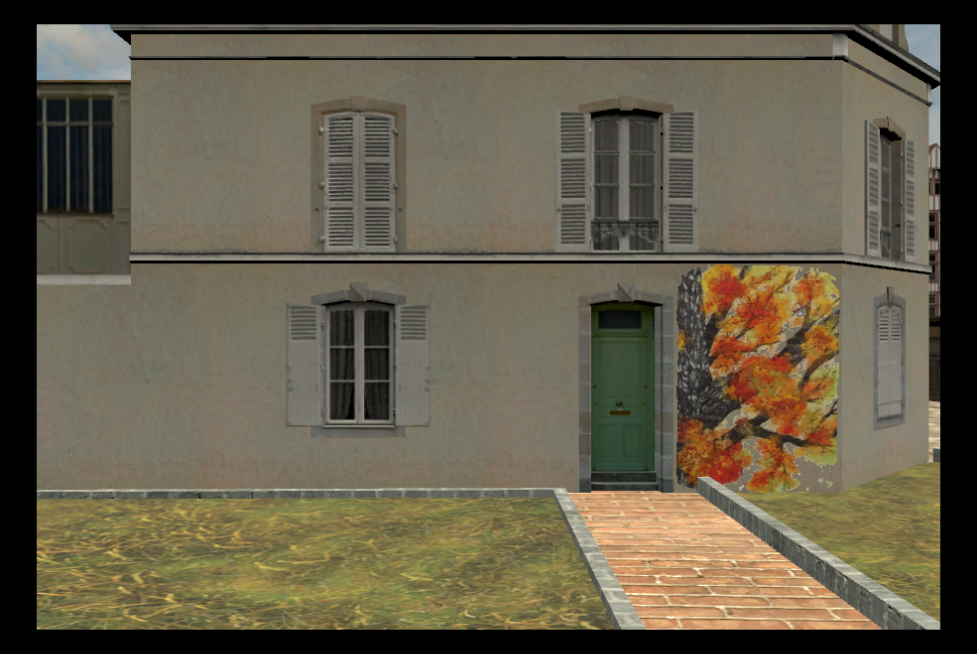
\includegraphics[width=\linewidth]{figures/54_R(tree)_noA.PNG}
		\caption{residential without human agent}
	\end{subfigure}

	\caption{Examples of photos shown in the pointing task as target buildings.}
	\label{fig:target_photos}
\end{figure}


Each trial was a pointing task performed from 28 different starting locations spread out through the city. At each starting location 12 consecutive trials were performed. In each trial a photo of one of the task buildings (with or without human agent in front of it) was presented at the top center of the screen. The participants had the option to press a button to bring the picture to the middle of the screen and as soon as they released the button the photo moved back to the upper center part of the screen. Since there was no visual virtual body, there was a green dashed laser beam attached to the virtual hand of the participants that moved as they moved their hand. The purpose of the laser beam was to assist the participants with the visualization of the direction they are pointing at. The maximum duration of each trial was 30 seconds. If there was no answer given to the task after 20 seconds from the start of the trial, i.e., no direction was selected by the participant indicating in which direction the target building is located from their current location, a countdown timer appeared on the bottom center of the screen and terminated the trial after 10 seconds if there was still no answer given. \\

Selecting an answer for the task, i.e., selecting the direction of the target building was possible with a button press. With once pressing the button it locked the laser beam onto a direction and detached it from the hand. The participants had the option to either confirm the chosen direction with the same button or cancel it with another. Moving on to the next trial was the result of either the participant confirming a direction or by running out of time. Behavioral and technical data, e.g., the chosen direction, participant position and rotation, reaction times were gathered during each trial. The human agents were present during the testing in the city at their exact designated positions and poses in the exploration sessions. A gray screen fade out and fade in occurred while transporting the participants from their current location to another starting location. This served the purpose of decreasing the chance of motion sickness and also avoiding leaking environmental information while moving in the city.

\todo{
	- include photo of the trial  \\
}


\section{Analysis method}

\todo{
	- the data is gathered in JSON format\\
	- preprocessing step (maybe with chart if applicable) \\
	- trial removal criteria (timeout) \\
	- check the assumptions for analysis? \\
	- linear mixed models (parameters: depvar='absolute\_180\_angles', subject='subject\_id', within=['starting\_loc\_id']) \\
	- linear mixed models (parameters: depvar='RT', subject='subject\_id', within=['starting\_loc\_id']) \\
	- maybe check for the effect of buildings as well
	- maybe other analysis methods
}

